

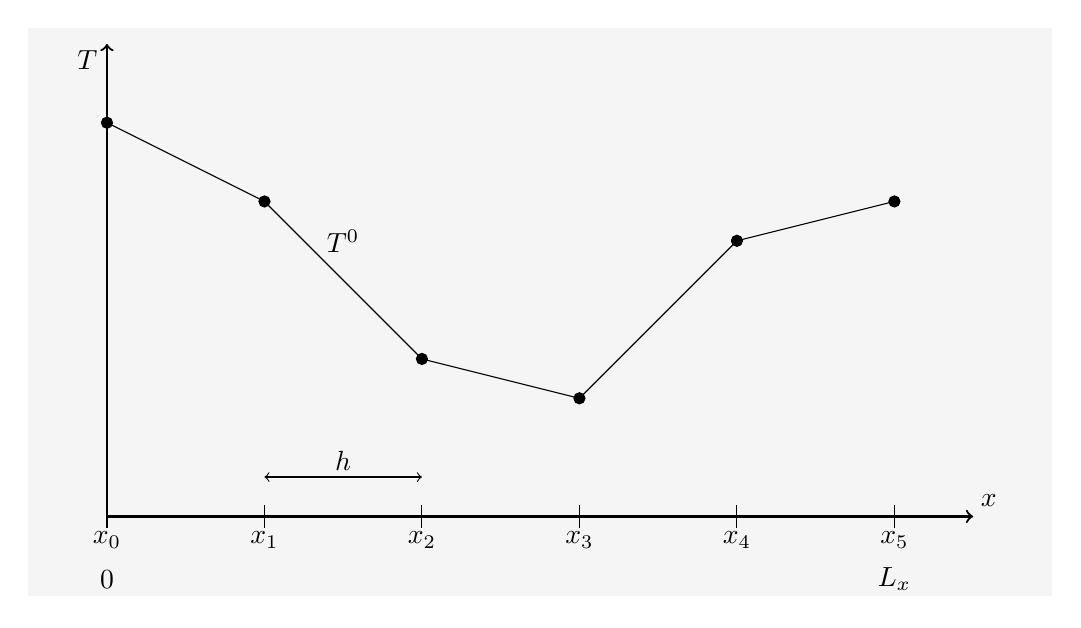
\begin{tikzpicture}
\draw[fill=gray!8,gray!8](0,0) rectangle (13,7.2);
%\draw[step=0.5cm,gray,very thin] (0,0) grid (13,7); %background grid

\draw[thick,->] (1,1) -- (12,1) ; 
\draw[thick,->] (1,1) -- (1,7) ; 


\node[] at (12.2,1.2) {$x$};
\node[] at (1,0.2) {$0$};
\node[] at (11,0.2) {$L_x$};
\node[] at (0.75,6.8) {$T$};

\draw[black,fill=black] (1,6)  circle (2pt);
\draw[black,fill=black] (3,5)  circle (2pt);
\draw[black,fill=black] (5,3)  circle (2pt);
\draw[black,fill=black] (7,2.5)  circle (2pt);
\draw[black,fill=black] (9,4.5)  circle (2pt);
\draw[black,fill=black] (11,5)  circle (2pt);

\draw[-] (1,6) -- (3,5) -- (5,3) -- (7,2.5) -- (9,4.5) -- (11,5); 
\node[] at (4,4.5) {$T^0$};

\draw[-] (1,0.85) -- (1,1.15) ; 
\draw[-] (3,0.85) -- (3,1.15) ; 
\draw[-] (5,0.85) -- (5,1.15) ; 
\draw[-] (7,0.85) -- (7,1.15) ; 
\draw[-] (9,0.85) -- (9,1.15) ; 
\draw[-] (11,0.85) -- (11,1.15) ; 
\node[] at (1,0.7) {$x_0$};
\node[] at (3,0.7) {$x_1$};
\node[] at (5,0.7) {$x_2$};
\node[] at (7,0.7) {$x_3$};
\node[] at (9,0.7) {$x_4$};
\node[] at (11,0.7) {$x_5$};
\draw[<->] (3,1.5) -- (5,1.5) ;  
\node[] at (4,1.7) {$h$};
\end{tikzpicture}

